\documentclass[
	openboth, % Capítulos começam em página direita
	oneside,   % Impressão frente e verso
	a4paper,   % Tamanho do papel
	english,   % Idioma adiciona para hifenizaçãoo
	brazil     % O ultimo é o idioma principal
]{abntex2}

\usepackage{lmodern}                               % Usa família de fontes Latin Modern
\usepackage[T1]{fontenc}                           % Codifição Type1 para a fonte (Fontes de 8 bits para incluir as fontes do alfabeto brasileiro)
\usepackage[UTF8]{inputenc}                        % Codificação unicode "UTF8"
\usepackage{microtype}                             % Melhorias na justificação (Evita bad/underfullbox)
\usepackage{indentfirst}                           % Indenta o primeiro parágrafo da seção
\usepackage{amssymb}                               % Símbolos matemáticos
\usepackage{enumitem}                              % Melhoria no suporte aos ambientes de numeração
\usepackage{color}                                 % Suporte a cores
\definecolor{blue}{RGB}{41,5,195}                  % Alterando o aspécto da cor Azul
\usepackage{graphicx}                              % Suporte a gráficos e figuras
\usepackage[alf]{abntex2cite}                      % Citações no padrão ABNT

% informações do PDF
\makeatletter
\hypersetup{
	%pagebackref=true,
	pdftitle={\@title}, 
	pdfauthor={\@author},
	pdfsubject={\imprimirpreambulo},
	pdfcreator={LaTeX with abnTeX2},
	pdfkeywords={abnt}{latex}{abntex}{abntex2}{trabalho acadêmico}, 
	colorlinks=true,       		% false: boxed links; true: colored links
	linkcolor=black,          	% color of internal links
	citecolor=black,        		% color of links to bibliography
	filecolor=black,      		% color of file links
	urlcolor=black,
	bookmarksdepth=4
}
\makeatother

% O tamanho do parágrafo é dado por:
\setlength{\parindent}{1.3cm}

% Controle do espaçamento entre um parágrafo e outro:
\setlength{\parskip}{0.2cm}  % tente também \onelineskip




\makeindex


\AtBeginDocument{
	\pagenumbering{gobble}
	\frenchspacing 
	\pretextual
	\tableofcontents*
	\textual
	\setlength\afterchapskip{\lineskip}
}

\begin{document}
	\begingroup
	\chapter{Introdução}
	\endgroup
	
	\pagenumbering{arabic}
	\setcounter{page}{1}
	
	As preocupações devido às emissões de CO2 tornaram a utilização de fontes de energias renováveis interessantes. Dentre elas, a energia baseada no vento se mostrou bastante promissora, pois o Brasil tem um dos maiores potenciais eólicos do mundo \cite{atlaseolico}.
	
	Com o aumento da participação da matriz eólica surgem novos desafios. A velocidade do vento é uma grandeza com grande variação instantânea, podendo variar bastante em questão de horas ou, até mesmo minutos. Essa variação, se não for contornada, pode trazer problemas de qualidade de energia, como a variação da frequência da rede devido a variação do vento, principalmente em redes mais fracas e dependentes da energia eólica. Além disso, há a presença de harmônicos devido ao movimento caótico do vento e ao efeito de sombra, ou seja, a perda de potência no momento em que uma das pás passa pela torre \cite{pintofundamentos}.
	
	Uma das soluções para melhorar a qualidade de energia de fontes eólicas é uso da eletrônica de potência em conjunto com topologias alternativas de geradores, como o GIDA (Gerador de indução duplamente alimentado).  A escolha do GIDA ocorre devido ao seu conversor processar até 30\% da potência nominal do gerador, enquanto em outros geradores com conversor acoplado esse valor chega a 100\%. Isto possibilita a redução do custo do conversor \cite{dattacomparacao,simoesrenewableinduction}. Nessa configuração tanto o estator quanto o rotor estão conectados à rede. Sendo o primeiro conectado diretamente (Figura \ref{figura:gida_esquematico}-A) e o rotor  é conectado através de uma derivação (Figura \ref{figura:gida_esquematico}-C), no qual existe um conversor CA/CA bidirecional \emph{back-to-back} \cite{heliodfig}.
	\begin{figure}[h]
		\centering
		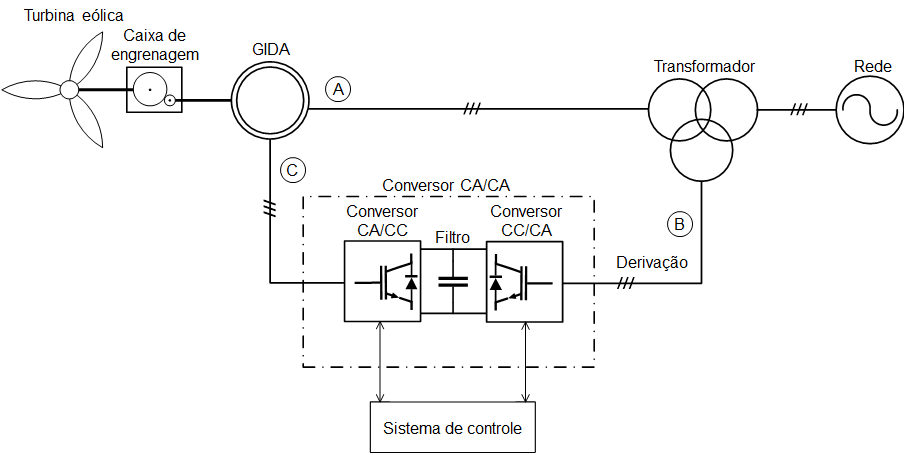
\includegraphics[width=1\textwidth]{Figuras/gida_esquematico.png}
		\caption{Esquema do GIDA conectado à rede para geração de energia eólica (Próprio autor).}
		\label{figura:gida_esquematico}
	\end{figure}

	O conversor \emph{back-to-back} é dividido em dois estágios. O primeiro converte a tensão alternada do lado voltado para a rede (Figura \ref{figura:gida_esquematico}-B) em tensão contínua, que é feita através do processo de retificação e com a ajuda de um filtro capacitivo, localizado logo após a saída deste estágio. Já o segundo estágio converte a tensão contínua novamente em tensão alternada, dessa vez aplicada ao rotor (Figura \ref{figura:gida_esquematico}-C). Esse processo é feito através da modulação por largura de pulso (PWM). Ambos os estágios são constituídos por pontes de \emph{Insulated Gate Bipolar Transistor} (IGBT), que são chaves semicondutoras para médias tensões. Dependendo de como as pontes de IGBT são chaveadas é possível regular a saída do conversor para tensões e frequências específicas \cite{alfeu}. 
	
	As técnicas de controle vetorial por orientação do fluxo do estator, ou de rotor, ou tensão de estator, permitem controlar separadamente as potências ativas e reativas do GIDA, além das grandezas de tensão e frequência. Essas técnicas consistem em controlar as componentes de eixo direto e em quadratura das correntes do rotor \cite{murilodq}. Inicialmente, utilizavam-se controladores proporcionais-integrais (PI) para este fim \cite{alfeu}. Mais recentemente, com o avanço dos sistemas computacionais e das técnicas de controle digital, surgiram novas alternativas como o \emph{deadbeat} \cite{deadbeat,deadbeatieee}, controle preditivo de matriz dinâmica de controle (DMC) \cite{dmcieee}, controle preditivo baseado em modelo (CPBM) \cite{alfeu,paperalfeu} e controle preditivo generalizado (GPC) \cite{gpcieee}. Todas elas apresentam excelente desempenho, porém a maioria dos trabalhos encontrados na literatura se limitam apenas a simulação.
	
	Devido ao estator do GIDA estar conectado diretamente à rede elétrica a ocorrência de afundamentos de tensão pode danificar os conversores que estão conectados aos enrolamentos do rotor. Inicialmente, a proteção empregada era um banco de resistores que eram ativados quando a falta era detectada \cite{rodrigo8afundamento,rodrigo9afundamento}. Com a evolução das técnicas de controle e modelagem matemática propostas como a apresentada em  \citeonline{rodrigo10afundamento} e \citeonline{rodrigo11afundamento} possibilitaram ao GIDA operar durante o afundamento de tensão com seu conversor operando.
	
	Sendo assim, este projeto de pesquisa tem o objetivo de preencher a lacuna existente na implementação do CPBM aplicado ao controle da potências do GIDA apresentado no trabalho de \citeonline{alfeu}. Possivelmente, também serão realizados testes do GIDA operando afundamentos de tensão. O sistema de controle será implementado no Laboratório de Eletrônica de Potência e Smart Grids da UFABC.
	
	\begingroup
	\let\clearpage\relax
	\chapter{Controle CPBM aplicado potências ativas e reativas do GIDA}
	\endgroup
	
	Os controladores preditivos levam em consideração o comportamento futuro do sistema, comparando a saída com a referência e encontrando uma função custo de menor valor possível \cite{camachoteoriapreditivomodelo,rositierteoriapreditivomodelo}. No CPBM é utilizado o modelo matemático do gerador de indução duplamente alimentado para fazer a predição das saídas futuras. Depois disso, é calculada a lei de controle através da minimização da função custo. A característica antecipativa do controle preditivo é desejável em sistemas onde há a mudança rápida de referência. Além disso, é possível lidar explicitamente com as restrições visto que estas podem ser incorporadas no processo de minimização da função custo \cite{alfeu}. A figura \ref{figura:preditivo_esquema} apresenta um diagrama representativo do sistema de controle preditivo.
	\begin{figure}[h]
		\centering
		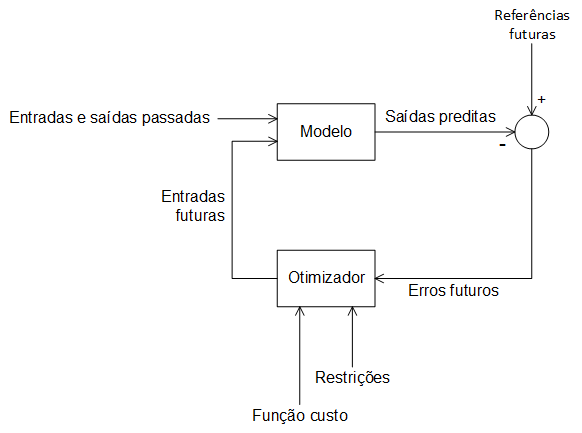
\includegraphics[width=0.5\textwidth]{Figuras/preditivo_esquematico.png}
		\caption{Diagrama representativo do sistema de controle preditivo \cite{alfeu}.}
		\label{figura:preditivo_esquema}
	\end{figure}

	Segundo \citeonline{geradorrefsinceq}, o modelo matemático do GIDA no referencial síncrono $dq$ girando com uma velocidade $\omega_1$ é dado por: 
	\begin{equation} 
		\label{equacao:gida_ref_sinc_estator}
		\vec{v}_{1dq}=R_1\vec{i}_{1dq}+\frac{d\vec{\lambda}_{1dq}}{dt}+j\omega_1\vec{\lambda}_{1dq}
	\end{equation}
	\begin{equation}
		\label{equacao_gida_ref_sinc_rotor}
		\vec{v}_{2dq}=R_2\vec{i}_{2dq}+\frac{d\vec{\lambda}_{2dq}}{dt}+j(\omega_1-n_p{\omega_{mec}})\vec{\lambda}_{2dq}
	\end{equation}
	A relação entre os fluxos concatenados em função das correntes são expressas por:
	\begin{equation}
		\label{equacao:gida_fluxo_estator}
		\vec{\lambda}_{1dq}=L_1\vec{i}_{1dq}+L_M\vec{i}_{2dq}
	\end{equation}
	\begin{equation}
		\label{equacao:gida_fluxo_rotor}
		\vec{\lambda}_{2dq}=L_M\vec{i}_{1dq}+L_2\vec{i}_{2dq}.
	\end{equation}
	e as potências ativas e reativas são dadas por:
	\begin{equation}
		\label{equacao:gida_potencia}
		P=\frac{3}{2}(v_{1d}i_{1d}+v_{1q}i_{1q})
	\end{equation}
	\begin{equation}
		\label{equacao:gida_reativo}
		Q=\frac{3}{2}(v_{1q}i_{1d}-v_{1d}i_{1q}).
	\end{equation}
	
	Nas equações \ref{equacao:gida_fluxo_estator} à \ref{equacao:gida_reativo} $\vec{v}$, $\vec{i}$ e $\vec{\lambda}$ são os vetores espaciais de tensão, corrente e fluxo magnético, respectivamente. Os subíndices 1 e 2 nas mesmas equações referem-se aos estator e rotor, respectivamente. E ainda, $R$ representa as resistências do estator e rotor por fase, $L$, as indutâncias próprias do estator e do rotor, $L_M$, a indutância mútua, $\omega_1$, a velocidade síncrona, $\omega_{mec}$, a velocidade mecânica e $n_p$, o número de pares de polos da máquina.
	
	O CPBM deste trabalho visa o controlar a potência ativa e reativa do estator através da regulação de fluxo do rotor. Ao adotar a orientação segundo o fluxo do estator o eixo direto é alinhado com vetor fluxo de estator, ou seja, $\lambda_{d1}=\lambda_1=|\lambda_{1dq}|$ e $\lambda_{1q}=0$ \cite{paperalfeu}. Utilizando-se deste fato e das equações \ref{equacao:gida_fluxo_estator} e \ref{equacao:gida_fluxo_rotor}, as equações \ref{equacao:gida_potencia} e \ref{equacao:gida_reativo} podem ser reescritas:
	\begin{equation}
		\label{equacao:gida_potencia_desacoplamento}
		P=-\frac{3v_1L_M}{2\sigma L_1L_2}\lambda_{2q}
	\end{equation}
	\begin{equation}
		\label{equacao:gida_reativo_desacoplamento}
		Q=\frac{3v_1L_M}{2\sigma L_1L_2}(-\lambda_{2d}+\frac{L_2}{L_M}\lambda_1).
	\end{equation}
	Onde  $v_1=v_{1q}=|\vec{v}_{1dq}|$ e $\sigma=1-(L_M^2)/(L_1L_2)$.
	
	A equação \ref{equacao_gida_ref_sinc_rotor} indica que o fluxo do rotor pode ser controlado através da tensão aplicada ao mesmo. Desprezando a resistência do rotor no cálculo da tensão em (\ref{equacao_gida_ref_sinc_rotor}), as potências ativas (\ref{equacao:gida_potencia_desacoplamento}) e reativas (\ref{equacao:gida_reativo_desacoplamento}) no referencial síncrono são iguais à:
	\begin{equation}
		\label{equacao:gida_reat_R}
		\frac{dQ(t)}{dt}=\frac{v_{d2}(t)}{A_m}+\omega_{sl}P(t)		
	\end{equation}
	\begin{equation}
		\label{equacao:gida_pot_R}
		\frac{dP(t)}{dt}=\frac{v_{2q}(t)}{A_m}+\omega_{sl}Q(t)-\omega_{s1}\frac{L_2}{L_MA_m}\lambda_1.
	\end{equation}
	Onde $\omega_{sl}=\omega_1-n_p\omega_{mec}$ e $A_m=-(2\sigma L_1L_2)/(3v_1L_m)$.
	
	Segundo \citeonline{ogata}, um sistema linear continuo no tempo pode ser representado por espaço de estados através da equação \ref{equacao:espaco_estados_continuo}. Onde $A$, $B$, $C$ e $G$ são matrizes $n \times n$, $\bar{x}$, o vetor de variáveis de estado, $\bar{u}$, o vetor de entradas, $\bar{y}$ o vetor de saídas e $\bar{w}$ o vetor de pertubações.
	\begin{equation}
		\label{equacao:espaco_estados_continuo}
		\begin{split}
			\dot{\bar{x}}=A\bar{x}+B\bar{u}+G\bar{w} \\
			\bar{y}=C\bar{x}
		\end{split}
	\end{equation}
	Reescrevendo as equações \ref{equacao:gida_reat_R} e \ref{equacao:gida_pot_R} na forma de espaço de estados (\ref{equacao:espaco_estados_continuo}), tem-se:
	\begin{equation}
		\label{equacao:espaco_estados_gida}
		\begin{bmatrix}
			\dot{Q} \\ \dot{P}
		\end{bmatrix} =
		\begin{bmatrix}
			0            & \omega_{sl} \\
			-\omega_{sl} & 0
		\end{bmatrix}
		\begin{bmatrix}
			Q \\
			P
		\end{bmatrix} + 
		\begin{bmatrix}
			\frac{1}{A_m} & 0 \\
			0 & \frac{1}{A_m}
		\end{bmatrix} + 
		\begin{bmatrix}
			1 & 0 \\
			0 & 1
		\end{bmatrix}
		\begin{bmatrix}
			0 \\
			-\omega_{sl}\frac{L_2}{L_mA_m}\lambda_1
		\end{bmatrix}
	\end{equation}
	Neste caso, as variáveis de estado são as próprias saídas do sistema, ou seja, a matriz C é igual a identidade.
	
	O sistema em (\ref{equacao:espaco_estados_gida}) não é linear, pois $\omega_{mec}$ varia com o tempo. Entretanto, a constante de tempo mecânica é muito maior que as constantes elétricas. Assim, considerando que o modelo será implementado em um sistema digital, portanto discreto no tempo. Pode-se fazer a linearização, considerando que $\omega_{mec}$ é aproximadamente constante para cada período de amostragem, $\omega_{sl}$ também é constante, visto que, $\omega_1=2\pi f$ é fixado pela frequência da rede, $f=60Hz$. 
	
	A discretização de (\ref{equacao:espaco_estados_gida}) em um período de amostragem $T$ através do \emph{zero-order-hold} (ZOH) sem atraso pode ser feita pela equação abaixo \cite{franklinpowell}:
	\begin{equation}
		\label{equacao:espaco_estados_discreto}
		\begin{split}
			\bar{x}(k+1)=A_d\bar{x}(k)+B_d\bar{u}(k)+G_d\bar{\omega}_d(k)
		\end{split}
	\end{equation}
	Onde:
	\begin{equation}
		\label{equacao:espaco_estados_discreto_matriz}
		\begin{split}
			A_d=e^{AT}\cong I+AT \\
			B_d=\int_0^\tau e^{AT}Bd\tau \cong BT \\
			G_d=\int_0^\tau e^{AT}Gd\tau \cong GT \\
			C_d = C
		\end{split}
	\end{equation}
	Substituindo (\ref{equacao:espaco_estados_gida}) em (\ref{equacao:espaco_estados_discreto}) e (\ref{equacao:espaco_estados_discreto_matriz}), tem-se:
	\begin{equation}
		\label{equacao:gida_espaco_estados_discreto}
		\begin{bmatrix}
			Q(k+1) \\
			P(k+1)
		\end{bmatrix} = 
		\begin{bmatrix}
			1             & \omega_{sl}T \\
			-\omega_{sl}T & 1
		\end{bmatrix}
		\begin{bmatrix}
			Q(k) \\
			P(k)
		\end{bmatrix} + 
		\begin{bmatrix}
			\frac{T}{A_m} & 0 \\
			0 & \frac{T}{A_m}
		\end{bmatrix}
		\begin{bmatrix}
			v_{2d}(k) \\
			v_{2q}(k)
		\end{bmatrix} +
		\begin{bmatrix}
			1 & 0 \\
			0 & 1 
		\end{bmatrix} 
		\begin{bmatrix}
			0 \\
			-\omega_{sl}\frac{L_2}{L_mA_mT}\lambda_1
		\end{bmatrix}
	\end{equation}
	
	A predição das saídas a partir do modelo matemático dinâmico da equação discretizada (\ref{equacao:gida_espaco_estados_discreto}) é dada por:
	\begin{equation}
		\label{equacao:predicao_saidas}
		Y=P_{px}\bar{x}(k)+HU+D\bar{\omega}_d(k)
	\end{equation}
	Onde:
	
	\bibliographystyle{abntex2-alf}
	\bibliography{biblio}
\end{document}